\section{Background}
\frame {
    \frametitle{Vector Boson Fusion (VBF)}

    \begin{columns}
        \begin{column}{0.5\textwidth}
            { \small VBF is the second highest Higgs production mechanism, but with a much cleaner signal than ggF }

            \begin{figure}
                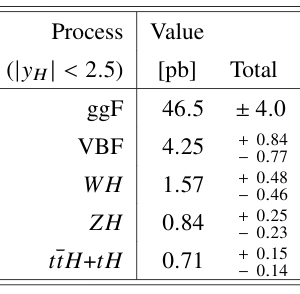
\includegraphics[width=\linewidth,height=0.5\textheight,keepaspectratio]{higgs_production_modes.png}
                \caption{\scriptsize source - arXiv:1909.02845 [hep-ex] }
            \end{figure}
        \end{column}
        \begin{column}{0.5\textwidth}
            {\scriptsize
                VBF jets have a recognizable signal as two hight-$p_T$ jets, with a large invariant mass and wide seperation in $\eta$.
            }
            %\resizebox{0.50\textheight}{!}{
                \begin{tikzpicture} \begin{feynman}
    \vertex (a);
    \vertex [right=of a] (b) {H};
    \vertex [above left=of a] (vb1);
    \vertex [below left=of a] (vb2);
    \vertex [left=of vb1] (q1i) {q};
    \vertex [left=of vb2] (q2i) {q};
    \vertex [above =of b] (q1f) {q};
    \vertex [below =of b] (q2f) {q};

    \diagram* {
        (q1i) -- (vb1) -- (q1f),
        (q2i) -- (vb2) -- (q2f), 
        (vb1) -- [boson] (a) -- [boson] (vb2),
        (a) -- [scalar] (b),
    };
\end{feynman} \end{tikzpicture}

                \begin{tikzpicture} \begin{feynman}
    \vertex (a);
    \vertex [right=of a] (b) {H};
    \vertex [above left=of a] (vb1);
    \vertex [below left=of a] (vb2);
    \vertex [left=of vb1] (q1i) {q};
    \vertex [left=of vb2] (q2i) {q};
    \vertex [above =of b] (q1f) {q};
    \vertex [below =of b] (q2f) {q};

    \diagram* {
        (q1i) -- (vb1) -- (q1f),
        (q2i) -- (vb2) -- (q2f), 
        (vb1) -- [boson] (a) -- [boson] (vb2),
        (a) -- [scalar] (b),
    };
\end{feynman} \end{tikzpicture}
 % replace with ggf...
            %}
        \end{column}
    \end{columns}
}

\frame {
    \frametitle{Two Jets are Simple}
    \begin{columns}
        \begin{column}{0.5\textwidth}
            \begin{tikzpicture} \begin{feynman}
    \vertex (a);
    \vertex [right=of a] (b) {H};
    \vertex [above left=of a] (vb1);
    \vertex [below left=of a] (vb2);
    \vertex [left=of vb1] (q1i) {q};
    \vertex [left=of vb2] (q2i) {q};
    \vertex [above =of b] (q1f) {q};
    \vertex [below =of b] (q2f) {q};

    \diagram* {
        (q1i) -- (vb1) -- (q1f),
        (q2i) -- (vb2) -- (q2f), 
        (vb1) -- [boson] (a) -- [boson] (vb2),
        (a) -- [scalar] (b),
    };
\end{feynman} \end{tikzpicture}

        \end{column}
        \begin{column}{0.5\textwidth}
        \end{column}
    \end{columns}




}

\frame {
    \frametitle{Three Jets Less So...}
    \begin{columns}
        \begin{column}{0.5\textwidth}
            \underline{\tiny Initial State Radiation (ISR)} \\
            \resizebox{0.50\textheight}{!}{
                \begin{tikzpicture} \begin{feynman}
    \vertex (a);
    \vertex [right=of a] (b) {H};
    \vertex [above left=of a] (vb1);
    \vertex [below left=of a] (vb2);
    \vertex [left=of vb1] (q1i) {q};
    \vertex [below left=of vb2] (q2k);
    \vertex [left=of q2k] (q2i) {q};
    \vertex [above =of b] (q1f) {q};
    \vertex [below =of b] (q2f) {q};
    \vertex [below =of q2f] (g) {g (ISR)};

    \diagram* {
        (q1i) -- (vb1) -- (q1f),
        (q2i) -- (q2k) -- (vb2) -- (q2f),
        (q2k) --[gluon] (g),
        (vb1) -- [boson] (a) -- [boson] (vb2),
        (a) -- [scalar] (b),
    };
\end{feynman} \end{tikzpicture}

            }
            \underline{\tiny Final State Radiation (FSR)} \\ 
            \resizebox{0.50\textheight}{!}{
                \begin{tikzpicture} \begin{feynman}
    \vertex (a);
    \vertex [right=of a] (b) {H};
    \vertex [above left=of a] (vb1);
    \vertex [below left=of a] (vb2);
    \vertex [left=of vb1] (q1i) {q};
    \vertex [left=of vb2] (q2i) {q};
    \vertex [below right=of vb2] (q2k);
    \vertex [above =of b] (q1f) {q};
    \vertex [below =of b] (q2f) {q};
    \vertex [below =of q2f] (g) {g (FSR)};

    \diagram* {
        (q1i) -- (vb1) -- (q1f),
        (q2i) -- (vb2) -- (q2k) -- (q2f), 
        (q2k) --[gluon] (g),
        (vb1) -- [boson] (a) -- [boson] (vb2),
        (a) -- [scalar] (b),
    };
\end{feynman} \end{tikzpicture}

            }
        \end{column}
        \begin{column}{0.5\textwidth}
        \end{column}
    \end{columns}
}
